% !TeX document-id = {7b84af01-1f7a-4dcf-8783-01201f47fbc1}
% !TeX TXS-program:compile = txs:///pdflatex/[--shell-escape]
\documentclass[a4paper, final]{article}
%\usepackage{literat} % Нормальные шрифты
\usepackage[14pt]{extsizes} % для того чтобы задать нестандартный 14-ый размер шрифта
\usepackage[T2A]{fontenc}
\usepackage[utf8]{inputenc}
\usepackage[russian]{babel}
\usepackage{amsmath}
\usepackage[left=25mm, top=20mm, right=20mm, bottom=20mm, footskip=10mm]{geometry}
\usepackage{ragged2e} %для растягивания по ширине
\usepackage{setspace} %для межстрочного интервала
\usepackage{moreverb} %для работы с листингами
\usepackage{indentfirst} % для абзацного отступа
\usepackage{moreverb} %для печати в листинге исходного кода программ
\renewcommand\verbatimtabsize{4\relax}
\renewcommand\listingoffset{0.2em} %отступ от номеров строк в листинге
\renewcommand{\arraystretch}{1.4} % изменяю высоту строки в таблице
\usepackage[font=small, singlelinecheck=false, justification=raggedleft, format=plain, labelsep=period]{caption} %для настройки заголовка таблицы
\usepackage{listings} %листинги
\usepackage{xcolor} % цвета
\usepackage{hyperref}% для гиперссылок
\usepackage{enumitem} %для перечислений
%\usepackage{pdflscape} %для pdf, хотя это не потребуется
%\usepackage{pdfpages} %для pdf, хотя это не потребуется
\usepackage{tikz}
\usepackage{graphicx}
\usepackage{float}
\usepackage{multirow}
\usepackage{makecell}
\usepackage{pdfpages}
\setlist[enumerate,itemize]{leftmargin=1.2cm} %отступ в перечислениях
\usepackage{minted}
\usemintedstyle{vs}
\usepackage{svg}


\hypersetup{colorlinks,
	allcolors=[RGB]{000 000 000}} %красивые гиперссылки (не красные)

\textheight=24cm % высота текста
\textwidth=16cm % ширина текста
\oddsidemargin=0pt % отступ от левого края
\topmargin=-1.5cm % отступ от верхнего края
\parindent=24pt % абзацный отступ
\parskip=0pt % интервал между абзацами
\tolerance=2000 % терпимость к "жидким" строкам
\flushbottom % выравнивание высоты страниц
\usepackage[justification=centering]{caption}
\usepackage{float}
\usepackage{minted}
\usemintedstyle{vs}
\definecolor{LightGray}{gray}{0.98}

\begin{document} % начало документа

% НАЧАЛО ТИТУЛЬНОГО ЛИСТА
\begin{center}
\hfill \break
\hfill \break
\normalsize{МИНИСТЕРСТВО НАУКИ И ВЫСШЕГО ОБРАЗОВАНИЯ РОССИЙСКОЙ ФЕДЕРАЦИИ\\
 федеральное государственное автономное образовательное учреждение высшего образования «Санкт-Петербургский политехнический университет Петра Великого»\\[10pt]}
\normalsize{институт компьютерных наук и кибербезопасности}\\[10pt] 
\normalsize{высшая школа технологий искусственного интеллекта}\\[10pt] 
\normalsize{Направление: 02.03.01 Математика и компьютерные науки}\\

\hfill \break
\hfill \break

\large{<<Технология разработки программного обеспечения>>}\\
\large{\textit{Построение функциональной модели}}\\
\large{\textit{<<Приложения выполнения унарных и бинарных операций}}\\
\large{\textit{над мультимножествами>> с помощью методологии IDEF0}}
\hfill \break

\hfill \break
\hfill \break
\end{center}
 
\small{ 
\begin{tabular}{lrrl}
\!\!\!Студент, & \hspace{2cm} & & \\
\!\!\!группы 5130201/20101 & \hspace{2cm} & \underline{\hspace{3cm}} &Астафьев И. Е. \\\\
\!\!\! & \hspace{2cm} & \\
\!\!\!Преподаватель & \hspace{2cm} & \underline{\hspace{3cm}} &  Курочкин М. А. \\\\
&&\hspace{5cm}
\end{tabular}
\begin{flushright}
<<\underline{\hspace{1cm}}>>\underline{\hspace{2.5cm}} 2024г.
\end{flushright}
}

\hfill \break
\hfill \break
\begin{center} \small{Санкт-Петербург, 2024} \end{center}
\thispagestyle{empty} % выключаем отображение номера для этой страницы

% КОНЕЦ ТИТУЛЬНОГО ЛИСТА

\tableofcontents

\newpage

\section* {Введение}
\addcontentsline{toc}{section}{Введение}
Постоянное усложнение производственно-технических и организационно - экономических систем – фирм, предприятий, производств, и др. субъектов производственно-хозяйственной деятельности - и необходимость их анализа с целью совершенствования функционирования и повышения эффективности обусловливают необходимость применения специальных средств описания и анализа таких систем. Эта проблема приобретает особую актуальность в связи с появлением интегрированных компьютеризированных производств и автоматизированных предприятий.


Для решения этой проблемы была разработана методология IDEF (\textbf{I}CAM \textbf{Def}inition), позволяющая исследовать структуру, параметры и характеристики производственно-технических и организационно-экономических систем. Общая методология IDEF состоит из трех частных методологий моделирования, основанных на графическом представлении систем:
\begin{itemize}
	\item \textbf{IDEF0} используется для создания \textbf{\textit{функциональной модели}}, отображающей структуру и функции системы, а также потоки информации и материальных объектов, связывающие эти функции.
	\item \textbf{IDEF1} применяется для построения \textbf{\textit{информационной модели}}, отображающей структуру и содержание  информационных потоков, необходимых для поддержки функций системы;
	\item \textbf{IDEF2} позволяет построить \textit{\textbf{динамическую модель}} меняющихся во времени поведения функций, информации и ресурсов системы.
\end{itemize}

В этом отчете описывается методология IDEF0, примененная к Приложению выполнения унарных и бинарных операций. 

\newpage
\section{Постановка задачи} 
\begin{enumerate}
	\item Изучить методологию IDEF0, основываясь на руководящем документе, утвержденном и введенном в действие Постановлением Госстандарта России от 2000 года. Это включает в себя изучение основных принципов и методов, используемых в IDEF0 для моделирования функциональных систем.
	\item Описать функциональную модель Приложения выполнения унарных и бинарных операций с помощью методологии IDEF0.
\end{enumerate}


\newpage
\section{Концепция IDEF0}
\textbf{IDEF0} используется для создания \textbf{функциональной модели}, отображающей структуру и функции системы, а также потоки информации и материальных объектов, связывающие эти функции.
Следующие концептуальные положения являются основой методологии IDEF0.

\par \textbf{Модель} -- искусственный объект, представляющий собой отображение (образ) системы и ее компонентов. Модель разрабатывают для понимания, анализа и принятия решений о реконструкции или замене существующей, либо проектировании новой системы. 
\par \textbf{Cистема} -- совокупность взаимосвязанных и взаимодействующих частей, выполняющих некоторую полезную работу. Частями (элементами) системы могут быть любые комбинации разнообразных сущностей, включающие людей, информацию, программное обеспечение, оборудование, изделия, сырье или энергию (энергоносители). Модель описывает, что происходит в системе, как ею управляют, какие сущности она преобразует, какие средства использует для выполнения своих функций и что производит.

\par \textbf{Блочное моделирование и его графическое представление} 
\par Основной концептуальный принцип методологии IDEF - представление любой изучаемой системы в виде набора взаимодействующих и взаимосвязанных блоков, отображающих процессы, операции, действия, происходящие в изучаемой системе. 
Функция -- все, что происходит в системе и ее элементах. Каждой функции ставится в соответствие блок. На IDEF0-диаграмме, основном документе при анализе и проектировании систем, блок представляет собой прямоугольник. Интерфейсы, посредством которых блок взаимодействует с другими блоками или с внешней по отношению к моделируемой системе средой, представляются стрелками, входящими в блок или выходящими из него. Входящие стрелки показывают, какие условия должны быть одновременно выполнены, чтобы функция, описываемая блоком, осуществилась.

\par \textbf{Лаконичность и точность} 
\par Документация, описывающая систему, должна быть точной и лаконичной. Многословные характеристики, изложенные в форме традиционных текстов, неудовлетворительны. Графический язык позволяет лаконично, однозначно и точно показать все элементы (блоки) системы и все отношения и связи между ними, выявить ошибочные, лишние или дублирующие связи и т.д..
\par \textbf{Передача информации} 
\par Средства IDEF0 облегчают передачу информации от одного участника разработки модели (отдельного разработчика или рабочей группы) к другому. К числу таких средств относятся:
\par- диаграммы, основанные на простой графике блоков и стрелок, легко читаемые и понимаемые;
\par- метки на естественном языке для описания блоков и стрелок, а также глоссарий и сопроводительный текст для уточнения смысла элементов диаграммы;
\par- последовательная декомпозиция диаграмм, строящаяся по иерархическому принципу, при котором на верхнем уровне отображаются основные функции, а затем происходит их детализация и уточнение;
\par- древовидные схемы иерархии диаграмм и блоков, обеспечивающие обозримость модели в целом и входящих в нее деталей.


\newpage
\par \textbf{Строгость и формализм} 
\par Разработка моделей IDEF0 требует соблюдения ряда строгих формальных правил, обеспечивающих преимущества
методологии в отношении однозначности, точности и целостности сложных многоуровневых моделей. Основное из них: все стадии и этапы разработки и корректировки модели должны строго, формально документироваться с тем, чтобы при ее эксплуатации не возникало вопросов, связанных с неполнотой или некорректностью документации.
\par \textbf{Итеративное моделирование} 
\par Разработка модели в IDEF0 представляет собой пошаговую, итеративную процедуру. На каждом шаге итерации разработчик предлагает вариант модели, который подвергают обсуждению, рецензированию и последующему редактированию, после чего цикл
повторяется. Такая организация работы способствует оптимальному использованию знаний системного аналитика, владеющего методологией и техникой IDEF0, и знаний специалистов – экспертов в предметной области, к которой относится объект моделирования.
\par \textbf{Отделение «организации» от «функций»}
\par При разработке моделей следует избегать изначальной «привязки» функций исследуемой системы к существующей организационной структуре моделируемого объекта (предприятия, фирмы). Это помогает избежать субъективной точки зрения, навязанной организацией и ее руководством. Организационная
структура должна явиться результатом использования (применения) модели. Сравнение результата с существующей структурой позволяет, во-первых, оценить адекватность модели, а во-вторых – предложить решения, направленные на совершенствование этой структуры.
\newpage
\section{Основные понятия методологии и языка IDEF0}
\par Методология IDEF0 предполагает создание иерархической системы диаграмм, представляющих собой единичные описания различных фрагментов системы. Сначала осуществляется общее описание системы и её взаимодействия с внешней средой через контекстную диаграмму. Затем проводится функциональная декомпозиция: система делится на подсистемы, каждая из которых описывается отдельно с помощью диаграмм декомпозиции. Этот процесс продолжается, пока каждая подсистема не будет разбита на более мелкие элементы, таким образом достигается необходимый уровень детализации.
\par \textbf{Диаграмма: }часть модели, описывающая декомпозицию блока.
\par \textbf{Модель IDEF0:} графическое описание системы, разработанное с определенной целью и с выбранной точки зрения. Комплект одной или более диаграмм IDEF0, которые изображают функции системы с помощью графики, текста и глоссария.

\par \textbf{Блок:} прямоугольник, содержащий имя и номер и используемый для описания функции.
\par \textbf{Ветвление:} разделение стрелки на два или большее число сегментов
\par \textbf{Входная стрелка:} класс стрелок, которые отображают вход IDEF0-блока, то есть данные или материальные объекты, которые преобразуются функцией в выход. Входные стрелки связываются с левой стороной блока IDEF0.
\par \textbf{Выходная стрелка: }класс стрелок, которые отображают выход IDEF0-блока, то есть данные или материальные объекты, произведенные функцией. Выходные стрелки связываются с правой стороной блока IDEF0.
\par \textbf{Декомпозиция:} разделение моделируемой функции на функции - компоненты.

\par \textbf{Контекст: }окружающая среда, в которой действует функция (или комплект функций на диаграмме).
\par \textbf{Контекстная диаграмма:} диаграмма, имеющая узловой номер A-n ( n $\geq$ 0 ), которая представляет контекст модели, Диаграмма A-0, состоящая из одного блока, является необходимой (обязательной) контекстной диаграммой; диаграммы с узловыми номерами A-1, A-2,... -- дополнительные контекстные диаграммы.

\par \textbf{Диаграмма A-0: } специальный вид (контекстной) диаграммы IDEF0, состоящей из одного блока, описывающего функцию верхнего уровня, ее входы, выходы, управления, и механизмы, вместе с формулировками цели модели и точки зрения, с которой строится модель. Каждая модель должна иметь контекстную диаграмму верхнего уровня, на которой объект моделирования представлен единственным блоком с граничными стрелками. Эта диаграмма называется A-0. Стрелки на этой диаграмме отображают связи объекта моделирования с окружающей средой. Поскольку единственный блок представляет весь объект, его имя -- общее для всего проекта. Это же справедливо и для всех стрелок диаграммы, поскольку они представляют полный комплект внешних интерфейсов объекта.

\par \textbf{Дочерняя диаграмма: } диаграмма, создаваемая при декомпозиции, охватывающая ту же область, что и родительский блок, но описывающая ее более подробно. Единственная функция, представленная на контекстной диаграмме верхнего уровня, может быть разложена на основные подфункции посредством создания дочерней диаграммы. В свою очередь, каждая из этих подфункций может быть разложена на составные части посредством создания дочерней диаграммы следующего, более низкого уровня, на которой некоторые или все функции также могут быть разложены на составные части. Каждая дочерняя диаграмма содержит дочерние блоки и стрелки, обеспечивающие дополнительную детализацию родительского блока.

\subsection{Компоненты синтаксиса}
Компоненты синтаксиса IDEF0 – блоки, стрелки, диаграммы и правила.
\par Блоки представляют функции, определяемые как деятельность, процесс, операция, действие или преобразование. Стрелки представляют данные или материальные объекты, связанные с функциями. Правила определяют, как следует применять компоненты; диаграммы обеспечивают формат графического и словесного описания моделей. Формат образует основу для управления конфигурацией модели.

\subsection{Диаграммы}
\par IDEF0-модели состоят из трех типов документов: графических диаграмм, текста и глоссария. Эти документы имеют перекрестные ссылки друг на друга. 
\par Графическая диаграмма – главный компонент IDEF0-модели, содержащий блоки, стрелки, соединения блоков и стрелок и ассоциированные с ними отношения. Блоки представляют основные функции моделируемого объекта. Эти функции могут быть разбиты (декомпозированы) на составные части и представлены в виде более подробных диаграмм; процесс декомпозиции продолжается до тех пор, пока объект не будет описан на уровне детализации, необходимом для достижения целей конкретного проекта. 
\par Диаграмма верхнего уровня обеспечивает наиболее общее или абстрактное описание объекта моделирования. 
\par За этой диаграммой следует серия дочерних диаграмм, дающих более детальное представление об объекте.


\par Процесс построения IDEF0-модели начинается с представления всей системы в виде простого компонента — одного блока, окруженного дугами, которые символизируют интерфейсы с внешними функциями. 


Представлена на Рис.\ref{fig:Контекстная диаграмма}.
\begin{center}
	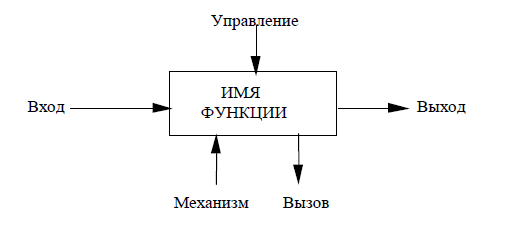
\includegraphics[scale=0.8]{context.png}
	\captionof{figure}{Контекстная диаграмма} 
	\label{fig:Контекстная диаграмма}
\end{center}

\par Затем этот блок, представляющий систему как единый модуль, детализируется на следующей диаграмме с использованием нескольких блоков, соединенных интерфейсными дугами. Эти блоки отображают основные подфункции (подмодули) исходного модуля.
\par Данная декомпозиция позволяет выявить полный набор подмодулей, каждый из которых представлен как отдельный блок, границы которого определены интерфейсными дугами. Каждый из этих подмодулей может быть далее декомпозирован аналогичным образом для более детального представления.

\par Структура IDEF0-модели представлена  на Рис.\ref{fig:Иерархия диаграмм}, где отображены четыре диаграммы и их взаимосвязи. 
\begin{center}
	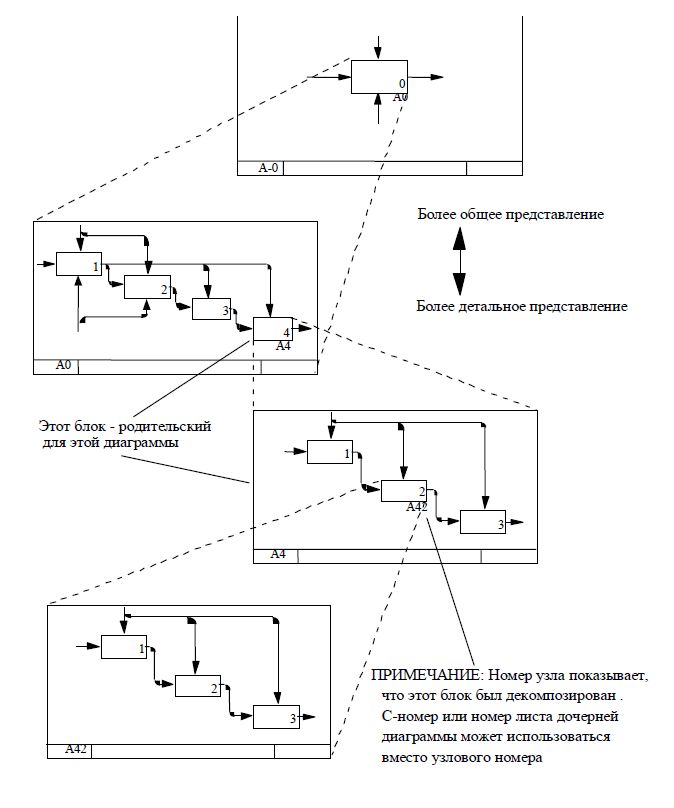
\includegraphics[scale=0.8]{ierarchy.png}
	\captionof{figure}{Иерархия диаграмм} 
	\label{fig:Иерархия диаграмм}
\end{center}


То, что блок является дочерним и раскрывает содержание родительского блока на диаграмме предшествующего уровня, указывается специальным ссылочным кодом, написанным ниже правого нижнего угла блока.



\newpage
\section{Модель IDEF0 для Приложения выполнения унарных и бинарных операций над мультимножествами}
\subsection{Контекстная диаграмма A-0}


\par Контекстная диаграмма A-0 для Приложения выполнения унарных и бинарных операций над мультимножествами представлена на Рис.\ref{fig1:Контекстная диаграмма А-0}. Точка зрения данной диаграммы: программист-разработчик. Она описывает функцию верхнего уровня, её входы, выходы, управления, и механизмы.
\begin{figure}[H]
	\centering
	\includesvg[width=\linewidth]{a-0}
	\captionof{figure}{Контекстная диаграмма А-0} 
	\label{fig1:Контекстная диаграмма А-0}
\end{figure}

Данная диаграмма задает основные параметры:
\begin{itemize}
\item Входные данные: техническое задание;
\item Выходные данные: разработанное приложение «Выполнение унарных и бинарных операций над мультимножествами»;
\item Управляющие данные: стандарт языка C++ 17 ISO/IEC;
\item Механизмы: программист, язык программирования C++.
\end{itemize}


\newpage
\subsection{Диаграмма А0}


\par Данная диаграмма является дочерней для контекстной диаграммы А-0 и представляет разбиение единственного блока реализации Приложения выполнения унарных и бинарных операций над мультимножествами и представлена на Рис.\ref{fig2:Диаграмма А0}.
\begin{figure}[H]
	\centering
	\includesvg[width=\linewidth]{a0}
	\captionof{figure}{Диаграмма А0} 
	\label{fig2:Диаграмма А0}
\end{figure}
\par На диаграмме были выделены следующие блоки:
\begin{enumerate}
\item Разработать класс, описывающий структуру универсума мультимножества;
\item Разработать класс, описывающий структуру мультимножества;
\item Дополнить класс мультимножества функциями выполнения операций над мультимножествами;
\item Разработать руководство оператора.
\end{enumerate}
Она дублирует следующие основные параметры с предыдущей диаграммы:
\begin{itemize}
\item Входные данные: техническое задание;
\item Выходные данные: разработанное приложение «Выполнение унарных и бинарных операций над мультимножествами»;
\item Управляющие данные: стандарт языка C++ 17 ISO/IEC;
\item Механизмы: программист, язык программирования C++.
\end{itemize}




\newpage
\subsection{Диаграмма А1}
\par Данная диаграмма является дочерней для А0 и представляет разбиение блока разработки класса, описывающего
структуру данных хэш-таблицы. Изображена на Рис.\ref{fig3:Диаграмма А1}. 

\begin{figure}[H]
	\centering
	\includesvg[width=\linewidth]{a1}
	\captionof{figure}{Диаграмма А1}
	\label{fig3:Диаграмма А1}
\end{figure}


\par На диаграмме были выделены следующие блоки:
\begin{enumerate}
\item Определить структуру хранения элементов универсума;
\item Реализовать функции вычисления кодов Грея;
\item Реализовать обработку ошибок;
\item Реализовать заполнение универсума.
\end{enumerate}
У этой диаграммы следующие основные параметры:
\begin{itemize}
\item Входные данные: ТЗ для элементов универсума и структуры класса универсума;
\item Выходные данные: реализованный класс, описывающий структуру универсума;
\item Управляющие данные: стандарт языка C++ 17 ISO/IEC;
\item Механизмы: программист, язык программирования C++.
\end{itemize}



\newpage
\subsection{Диаграмма А2}
\par Данная диаграмма является дочерней для А0 и представляет разбиение блока разработки функций, позволяющих выполнять операции с хэш-таблицей. Изображена на Рис.\ref{fig4:Диаграмма А2}. 

\begin{figure}[H]
	\centering
	\includesvg[width=\linewidth]{a2}
	\captionof{figure}{Диаграмма А2} 
	\label{fig4:Диаграмма А2}
\end{figure}


\par На диаграмме были выделены следующие блоки:
\begin{enumerate}
\item Определить базовую структуру класса мультимножества;
\item Реализовать функцию заполнения мультимножества.
\end{enumerate}
У этой диаграммы следующие основные параметры:
\begin{itemize}
\item Входные данные: ТЗ для структуры класса мультимножества;
\item Выходные данные: реализованный класс, описывающий структуру мультимножества;
\item Управляющие данные: стандарт языка C++ 17 ISO/IEC;
\item Механизмы: программист, язык программирования C++.
\end{itemize}


\newpage
\subsection{Диаграмма А3}
\par Данная диаграмма является дочерней для А0 и представляет разбиение блока разработки функций, позволяющих выполнять операции с хэш-таблицей. Изображена на Рис.\ref{fig4:Диаграмма А3}. 

\begin{figure}[H]
	\centering
	\includesvg[width=\linewidth]{a3}
	\captionof{figure}{Диаграмма А3} 
	\label{fig4:Диаграмма А3}
\end{figure}


\par На диаграмме были выделены следующие блоки:
\begin{enumerate}
\item Реализовать функцию дополнения мультимножества;
\item Реализовать функции разностей и симметрической разности мультимножества;
\item Реализовать функции пересечения и объединения мультимножества;
\item Реализовать функции умножения и деления мультимножества;
\item Реализовать функции сложения и вычитания мультимножества;
\item Собрать все реализованные функции в классе мультимножества.
\end{enumerate}
У этой диаграммы следующие основные параметры:
\begin{itemize}
\item Входные данные: ТЗ для реализации функций работы с мультимножествами;
\item Выходные данные: класс с функциями, позволяющими выполнять операции с мультимножествами;
\item Управляющие данные: стандарт языка C++ 17 ISO/IEC;
\item Механизмы: программист, язык программирования C++.
\end{itemize}



\newpage
\section*{Заключение}

\addcontentsline{toc}{section}{Заключение}
В ходе выполнения данной работы была детально изучена методология IDEF0. Разработана функциональная модель Приложения выполнения унарных и бинарных операций над мультимножествами с применением методологии IDEF0. Созданы четыре диаграммы, которые структурировали и формализовали процесс разработки. Построена контекстная диаграмма A-0, проведена её декомпозиция и созданы три дочерние диаграммы: А0, А21, А2, A3. Они позволяют получить чёткое представление о функциональных аспектах Приложения и помогают анализировать взаимодействие компонентов системы.


\newpage
\addcontentsline{toc}{section}{Список использованной литературы}
\begin{thebibliography}{}
	\bibitem{litlink1} ГОССТАНДАРТ РОССИИ. Руководящий документ. МЕТОДОЛОГИЯ ФУНКЦИОНАЛЬНОГО МОДЕЛИРОВАНИЯ IDEF0. Москва: ИПК Издательство стандартов,
	2000г., 75с.
\end{thebibliography}
\thispagestyle{empty}

\newpage
\end{document}